\begin{figure}[t]
\centering
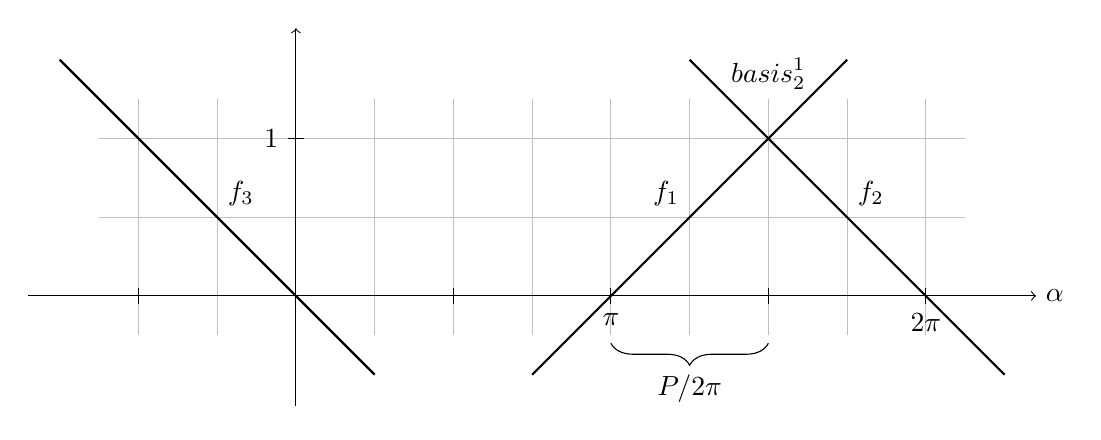
\begin{tikzpicture}
  \draw[color=lightgray] (-2.5, -0.5) grid (8.5, 2.5);

  \draw[thick] (3, -1) -- node[shift={(-0.3,0.3)}] {$f_1$} (7, 3);
  \draw[thick] (9, -1) -- node[shift={(0.3,0.3)}]  {$f_2$} (5, 3);
  \draw[thick] (1, -1) -- node[shift={(0.3,0.3)}]  {$f_3$} (-3, 3);

  \draw[->] (-3.4, 0) -- (9.4, 0) node[right] {$\alpha$};
  \draw[->] (0, -1.4) -- (0, 3.4);
  \draw (0.1, 2) -- (-0.1, 2) node[left] {$1$};
  \draw (-2, 0.1) -- (-2, -0.1);
  \draw (2, 0.1) -- (2, -0.1);
  \draw (4, 0.1) -- (4, -0.1) node[below] {$\pi$};
  \draw (6, 0.1) -- (6, -0.1);
  \draw (8, 0.1) -- (8, -0.1) node[below] {$2\pi$};

  \draw (6,2.5) node[above] {$\gls{basis}_2^1$};

  \draw [decoration={brace,mirror,amplitude=8pt},decorate] (4,-0.6) -- node[below=8pt] {$P/2\pi$} (6,-0.6);
\end{tikzpicture}
\caption[B-Spline-Funktion mit $K=1$ über Minimum-Maximumfunktion]{Beweisidee zur \enquote{kreisförmigen} Dreiecksfunktion für B-Spline-Funktionen mit $K=1$ und $P=4$ als Darstellung über eine Mi\-ni\-mum-Ma\-xi\-mum\-funk\-ti\-on auf drei Geraden, hier illustriert am Beispiel $\gls{basis}_2^1$.}
\label{fig:bspline_beweis}
\end{figure}
